\documentclass[letterpaper, 11pt]{extarticle}
% \usepackage{fontspec}

% ==================================================

% document parameters
% \usepackage[spanish, mexico, es-lcroman]{babel}
\usepackage[english]{babel}
\usepackage[margin = 1in]{geometry}

% ==================================================

% Packages for math
\usepackage{mathrsfs}
\usepackage{amsfonts}
\usepackage{amsmath}
\usepackage{amsthm}
\usepackage{amssymb}
\usepackage{physics}
\usepackage{dsfont}
\usepackage{esint}

% ==================================================

% Packages for writing
\usepackage{enumerate}
\usepackage[shortlabels]{enumitem}
\usepackage{framed}
\usepackage{csquotes}

% ==================================================

% Miscellaneous packages
\usepackage{float}
\usepackage{tabularx}
\usepackage{xcolor}
\usepackage{multicol}
\usepackage{subcaption}
\usepackage{caption}
\usepackage{appendix}
\captionsetup{format = hang, margin = 10pt, font = small, labelfont = bf}

% Citation
\usepackage[round, authoryear]{natbib}

% Hyperlinks setup
\usepackage{hyperref}
\definecolor{links}{rgb}{0.36,0.54,0.66}
\hypersetup{
   colorlinks = true,
    linkcolor = black,
     urlcolor = blue,
    citecolor = blue,
    filecolor = blue,
    pdfauthor = {Author},
     pdftitle = {Title},
   pdfsubject = {subject},
  pdfkeywords = {one, two},
  pdfproducer = {LaTeX},
   pdfcreator = {pdfLaTeX},
   }
\usepackage{titlesec}
\usepackage[many]{tcolorbox}

% Adjust spacing after the chapter title
\titlespacing*{\chapter}{0cm}{-2.0cm}{0.50cm}
\titlespacing*{\section}{0cm}{0.50cm}{0.25cm}

% Indent 
\setlength{\parindent}{0pt}
\setlength{\parskip}{1ex}

% --- Theorems, lemma, corollary, postulate, definition ---
% \numberwithin{equation}{section}

\newtcbtheorem[]{problem}{Problem}%
    {enhanced,
    colback = black!5, %white,
    colbacktitle = black!5,
    coltitle = black,
    boxrule = 0pt,
    frame hidden,
    borderline west = {0.5mm}{0.0mm}{black},
    fonttitle = \bfseries\sffamily,
    breakable,
    before skip = 3ex,
    after skip = 3ex
}{problem}

\tcbuselibrary{skins, breakable}

% --- You can define your own color box. Just copy the previous \newtcbtheorm definition and use the colors of yout liking and the title you want to use.
% --- Basic commands ---
%   Euler's constant
\newcommand{\eu}{\mathrm{e}}

%   Imaginary unit
\newcommand{\im}{\mathrm{i}}

%   Sexagesimal degree symbol
\newcommand{\grado}{\,^{\circ}}

% --- Comandos para álgebra lineal ---
% Matrix transpose
\newcommand{\transpose}[1]{{#1}^{\mathsf{T}}}

%%% Comandos para cálculo
%   Definite integral from -\infty to +\infty
\newcommand{\Int}{\int\limits_{-\infty}^{\infty}}

%   Indefinite integral
\newcommand{\rint}[2]{\int{#1}\dd{#2}}

%  Definite integral
\newcommand{\Rint}[4]{\int\limits_{#1}^{#2}{#3}\dd{#4}}

%   Dot product symbol (use the command \bigcdot)
\makeatletter
\newcommand*\bigcdot{\mathpalette\bigcdot@{.5}}
\newcommand*\bigcdot@[2]{\mathbin{\vcenter{\hbox{\scalebox{#2}{$\m@th#1\bullet$}}}}}
\makeatother

%   Hamiltonian
\newcommand{\Ham}{\hat{\mathcal{H}}}

%   Trace
\renewcommand{\Tr}{\mathrm{Tr}}

% Christoffel symbol of the second kind
\newcommand{\christoffelsecond}[4]{\dfrac{1}{2}g^{#3 #4}(\partial_{#1} g_{#2 #4} + \partial_{#2} g_{#1 #4} - \partial_{#4} g_{#1 #2})}

% Riemann curvature tensor
\newcommand{\riemanncurvature}[5]{\partial_{#3} \Gamma_{#4 #2}^{#1} - \partial_{#4} \Gamma_{#3 #2}^{#1} + \Gamma_{#3 #5}^{#1} \Gamma_{#4 #2}^{#5} - \Gamma_{#4 #5}^{#1} \Gamma_{#3 #2}^{#5}}

% Covariant Riemann curvature tensor
\newcommand{\covariantriemanncurvature}[5]{g_{#1 #5} R^{#5}{}_{#2 #3 #4}}

% Ricci tensor
\newcommand{\riccitensor}[5]{g_{#1 #5} R^{#5}{}_{#2 #3 #4}}
\usepackage{listings}
\usepackage{xcolor}
\lstset{
  language=Python,
  basicstyle=\ttfamily\small,  % Police monospace petite
  frame=lines,                % Cadre autour du code
  numbers=left,               % Numéros de ligne
  keywordstyle=\color{blue},  % Couleur des mots-clés
  commentstyle=\color{green!50!black}, % Couleur des commentaires
  stringstyle=\color{red},    % Couleur des chaînes
  breaklines=true,            % Coupe les longues lignes
}

\begin{document}

\begin{Large}
    \textsf{\textbf{Stochastic Linear Bandits}}
    An Empirical Study
\end{Large}

\vspace{1ex}

\textsf{\textbf{Students:}} \text{Alexis Marouani, Grégoire Béchade}, \\
\textsf{\textbf{Lecturer:}} \text{Claire Vernade}, Contact me on Slack if anything looks weird, or find my email on my \href{www.cvernade.com}{website} 

\section{Problem 1: Linear epsilon greedy}

\begin{enumerate}
    \item For LinUCB, here is the code of our receive\_reward function with the updates of the covariance matrix. The action is then chosen as the maximizer of the inner product between the estimated $\hat{\theta}$ and the arms.

    \begin{lstlisting}[language=Python]

        
  def receive_reward(self, chosen_arm, reward):
    """
    update the internal quantities required to estimate the parameter theta using least squares
    """
    #update inverse covariance matrix
    self.cov += np.outer(chosen_arm, chosen_arm) # update the covariance matrix
    self.invcov = pinv(self.cov) # update the inverse covariance matrix

    #update b_t
    self.b_t += reward * chosen_arm

    self.hat_theta = np.inner(self.invcov, self.b_t) # update the least square estimate
    self.t += 1
    \end{lstlisting}


        
    \item q2
    \item According to the documentation of numpy, the complexity of the pinv function is $O(min(n m^2, n^2m))$. In our problem, the matrix is squared, of size $d$ so the complexity is $O(d^3)$.
This can create problems when facing high-dimensional problems. We have therefore decided to implement a class LinearEpsilonGreedybis, in which we have changed the estimation of $\hat{\theta}$. 
Instead of estimating $\theta$ through the least square estimator, we decided to estimate it through this estimator: $\hat{\theta} = \sum_{t=1}^{T} \left\langle \theta , A_t\right\rangle A_t$. 
We didn't manage to find theoretical guarantees about the expected value of this estimator, as $\mathbb{E}(\hat{\theta}) = \sum_{t=1}^{T} \mathbb{E} ( \left\langle \theta , A_t\right\rangle A_t) $, which can't be precised without assumptions on the distribution of $A_t$.
However, we have tested it on different problems, and it seems to obtain the same results as the one obtained with the least square estimator.
Computing $\hat{\theta}$ has a complexity in $0(d)$, as we only have to compute scalars products of d-vectors. The figure \ref{fig:lin_epsilon_greedy} underlines the gain in computational time, while the performances are the same.

\begin{figure}[h]
    \centering
    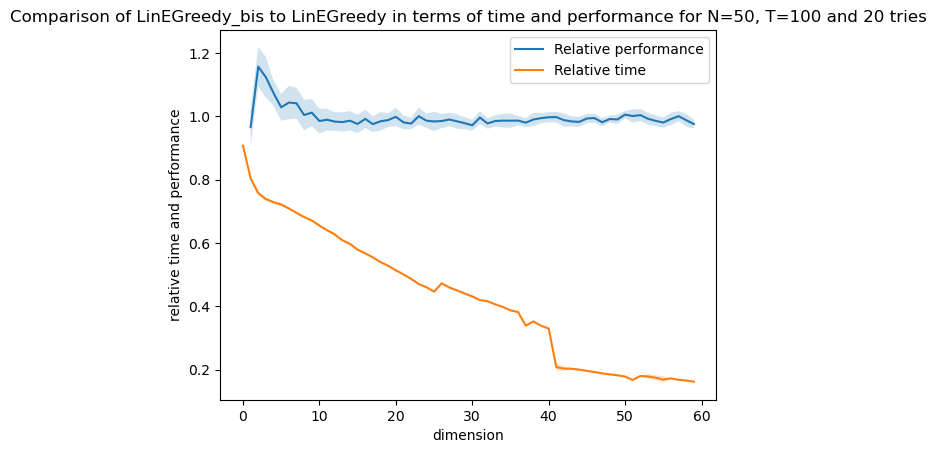
\includegraphics[width=0.5\textwidth]{images/comparison.png}
    \caption{Comparison of the performances and time of execution of LinearEpsilonGreedy and the LinearEpsilonGreedy bis, with N=50, T=200 and 20 tries.} 
    \label{fig:lin_epsilon_greedy}
\end{figure}





\end{enumerate}


\section{Problem 2: LinUCB and LinTS}


\begin{enumerate}
    \item For the implementation of LinUCB, we have implemented the function $\beta(t,\delta)$ and directly computed the upper confidence born from the course. The arm selected is the one that maximises the following quantity: \\
     $x^T\hat{\theta }^\lambda _t + \left\lVert x\right\rVert _{(B_t^\lambda)^{-1} } \beta(t, \delta) $. 

    For the LinTS, we update the parameters as described in q2. We then draw a $\theta^*$ from the posterior distribution and choose the arm that maximizes the inner product between the arm and the sampled $\theta^*$.
    We provide the code of the get\_action function below.
    \begin{lstlisting}
        
  def get_action(self, arms):
    theta= np.random.multivariate_normal(self.mu, self.cov)
    theta=theta/np.linalg.norm(theta)
    return arms[np.argmax(np.dot(arms, theta))]
    \end{lstlisting}
    \item The prior on $\theta^*$ is that it follows the law $\mathcal{N}(0, \Sigma)$. \\
    
Let us define : \\
$\Sigma_t ^{-1} = \Sigma^{-1} + \frac{\sum_{t=1}^{T} A_t^T A_t}{\sigma^2}$ \\

and $\mu_t = \Sigma_t \times (\frac{\sum_{t=1}^{T} A_t^T r_t}{\sigma^2})$


The posterior on  $\theta^*$ is  $\mathcal{N}(\mu_t, \Sigma_t)$
    \item q3
\end{enumerate}

\section{Appendix}

\textbf{Proof of the posterior distribution of $\theta^*$ in LinTS}


Let us note  $A_t$, the chosen action at time $t$ and $Y_t = < A_t, \theta^*> + \epsilon_t$ the reward. 

We directly have that, $Y_t \sim \mathcal{N}(A_t (\theta^*) ^T, \sigma^2)$. 

Thanks to Bayes rule, we have : \\

$\mathbb{P}(\theta^* | Y_1, ... , Y_t , A_1, ..., A_t) = \mathbb{P}( Y_1, ... , Y_t , A_1, ..., A_t | \theta^* ) \times \frac{\mathbb{P}(\theta^*)}{\mathbb{P}(Y_1, ... , Y_t , A_1, ..., A_t) } $

The denominator is a constant with respect to $\theta^*$ so :

$\mathbb{P}(\theta^* | Y_1, ... , Y_t , A_1, ..., A_t) \propto \mathbb{P}( Y_1, ... , Y_t , A_1, ..., A_t | \theta^* ) \times {\mathbb{P}(\theta^*)}$ 

But, $\theta^* \sim \mathcal{N}(0, \Sigma)$ and

$\mathbb{P}( Y_1, ... , Y_t , A_1, ..., A_t | \theta^* ) = \Pi_{t=1}^{T} \frac{1}{\sqrt{2  \pi}} exp(\frac{-1}{2 \sigma^2} (A_t {\theta^*}^T -r_t)^2) = (\frac{1}{\sqrt{2  \pi}})^T \times exp(\sum_{t=1}^T\frac{-1}{2 \sigma^2} (A_t {\theta^*}^T -r_t)^2) $


$\theta^*$ and $(Y_1, ... , Y_t , A_1, ..., A_t | \theta^*)$ follow normal distributions so  $\theta^* | Y_1, ... , Y_t , A_1, ..., A_t$ also follows a normal distribution.  
We finally just have to identify the mean ($\mu_t$) and the covariance matrix ($\Sigma_t$) of this distribution. 

\begin{align}
    log (\mathbb{P}((  \theta^* |Y_1, ... , Y_t , A_1, ..., A_t ))) &= C + \sum_{t=1}^T\frac{-1}{2 \sigma^2} (A_t {\theta^*}^T -r_t)^2 -\frac{1}{2}({\theta^*}^T \Sigma ^{-1} \theta^*)\\
    & =\frac{-1}{2} ( (\sum_{t=1}^T \frac{(A_t^T {\theta^*}^T \theta^* A_t - 2 r_t A_t{\theta^*}^T + r_t^2)}{\sigma^2}) + {\theta^*}^T \Sigma ^{-1} \theta^*) +C\\
    & = C + {\theta^* }^T(\frac{1}{\sigma^2}\sum_{t=1}^{T} A_t^T A_t + \Sigma^{-1}) \theta^* - 2 {\theta^* }^T(\frac{\sum_{t=1}^T A_t r_t} {\sigma^2}) -(\frac{r_t}{\sigma})^2\\
\end{align}

We finally identify $\Sigma_t$ thanks to the quadratic term in $\theta^*$ :


$\Sigma_t ^{-1} = \Sigma^{-1} + \frac{\sum_{t=1}^{T} A_t^T A_t}{\sigma^2}$ 

and we have directly $\mu_t = \Sigma_t \times (\frac{\sum_{t=1}^{T} A_t^T r_t}{\sigma^2})$. 


\end{document}